\documentclass{article}
\usepackage{graphicx}
\usepackage{color}

\sloppy
\definecolor{lightgray}{gray}{0.5}
\setlength{\parindent}{0pt}

\begin{document}

    
    
\section*{}


\subsection*{Contents}

\subsection*{a) Plot the training data}

\begin{verbatim}
plot(Xtr(1:20),Ytr(1:20),'bo');
hold on
title('Plotting the First 20 Training Data Points');
\end{verbatim}

\includegraphics [width=4in]{practice1_01.eps}


\subsection*{b) Create a linear regression learn using the above functions}

\begin{verbatim}
Xtr_2 = [ ones(size(Xtr,1) ,1) , Xtr , Xtr.^2];
learner = linearReg(Xtr_2 ,Ytr); % train a linear regression learner


% plot it on the same plot as the training data
xline = [0:.01:1]';
yline = predict( learner , polyx (xline ,2) );
plot(xline, yline, 'r*');
legend('Training Data','Linear Regression');
\end{verbatim}

\includegraphics [width=4in]{practice1_02.eps}


\subsection*{c) Create plots with the data and a higher-order polynomial}



\subsection*{3}

\begin{verbatim}
Xtr_3 = [ ones(size(Xtr,1) ,1) , Xtr , Xtr.^2, Xtr.^3];
Xte_3 = [ ones(size(Xte,1) ,1) , Xte , Xte.^2, Xte.^3];

learner = linearReg(Xtr_3 ,Ytr); % train a linear regression learner

yline = predict( learner , polyx (xline ,3) );

% plot it on the same plot as the training data
figure
plot(Xtr(1:20),Ytr(1:20),'bo');
hold on
title('Data and linear regression of 3rd order');
plot(xline, yline, 'r*');
legend('Training Data','Linear Regression');

disp('Training MSE of order 3 regression')
tr_err = mse(learner,Xtr_3,Ytr)
disp('Testing MSE of order 3 regression')
te_err = mse(learner,Xte_3, Yte)
disp('MAE for order 3 regression')
te_mae = mae(learner,Xte_3, Yte)
\end{verbatim}


\subsection*{5}

\begin{verbatim}
Xtr_3 = [ ones(size(Xtr,1) ,1) , Xtr , Xtr.^2, Xtr.^3, Xtr.^4, Xtr.^5];
Xte_3 = [ ones(size(Xte,1) ,1) , Xte , Xte.^2, Xte.^3, Xte.^4, Xte.^5];

learner = linearReg(Xtr_3 ,Ytr); % train a linear regression learner

yline = predict( learner , polyx (xline ,5) );

% plot it on the same plot as the training data
figure
plot(Xtr(1:20),Ytr(1:20),'bo');
hold on
title('Plotting data and linear regression of 5th order');
plot(xline, yline, 'r*');
legend('Training Data','Linear Regression');

disp('Training MSE of order 5 regression')
tr_err = mse(learner,Xtr_3,Ytr)
disp('Testing MSE of order 5 regression')
te_err = mse(learner,Xte_3, Yte)
disp('MAE for order 5 regression')
te_mae = mae(learner,Xte_3, Yte)
\end{verbatim}


\subsection*{7}

\begin{verbatim}
Xtr_3 = [ ones(size(Xtr,1) ,1) , Xtr , Xtr.^2, Xtr.^3, Xtr.^4, Xtr.^5, Xtr.^6, Xtr.^7];
Xte_3 = [ ones(size(Xte,1) ,1) , Xte , Xte.^2, Xte.^3, Xte.^4, Xte.^5, Xte.^6, Xte.^7];

learner = linearReg(Xtr_3 ,Ytr); % train a linear regression learner

yline = predict( learner , polyx (xline ,7) );

% plot it on the same plot as the training data
figure
plot(Xtr(1:20),Ytr(1:20),'bo');
hold on
title('Plotting data and linear regression of 7th order');
plot(xline, yline, 'r*');
legend('Training Data','Linear Regression');

disp('Training MSE of order 7 regression')
tr_err = mse(learner,Xtr_3,Ytr)
disp('Testing MSE of order 7 regression')
te_err = mse(learner,Xte_3, Yte)
disp('MAE for order 7 regression')
te_mae = mae(learner,Xte_3, Yte)
\end{verbatim}


\subsection*{9}

\begin{verbatim}
Xtr_3 = [ ones(size(Xtr,1) ,1) , Xtr , Xtr.^2, Xtr.^3, Xtr.^4, Xtr.^5, Xtr.^6, Xtr.^7, Xtr.^8, Xtr.^9];
Xte_3 = [ ones(size(Xte,1) ,1) , Xte , Xte.^2, Xte.^3, Xte.^4, Xte.^5, Xte.^6, Xte.^7, Xte.^8, Xte.^9];

learner = linearReg(Xtr_3 ,Ytr); % train a linear regression learner

yline = predict( learner , polyx (xline ,9) );

% plot it on the same plot as the training data
figure
plot(Xtr(1:20),Ytr(1:20),'bo');
hold on
title('Plotting data and linear regression of 9th order');
plot(xline, yline, 'r*');
legend('Training Data','Linear Regression');

disp('Training MSE of order 9 regression')
tr_err = mse(learner,Xtr_3,Ytr)
disp('Testing MSE of order 9 regression')
te_err = mse(learner,Xte_3, Yte)
disp('MAE for order 9 regression')
te_mae = mae(learner,Xte_3, Yte)
\end{verbatim}


\subsection*{11}

\begin{verbatim}
Xtr_3 = [ ones(size(Xtr,1) ,1) , Xtr , Xtr.^2, Xtr.^3, Xtr.^4, Xtr.^5, Xtr.^6, Xtr.^7, Xtr.^8, Xtr.^9,  Xtr.^10, Xtr.^11];
Xte_3 = [ ones(size(Xte,1) ,1) , Xte , Xte.^2, Xte.^3, Xte.^4, Xte.^5, Xte.^6, Xte.^7, Xte.^8, Xte.^9,  Xte.^10, Xte.^11];

learner = linearReg(Xtr_3 ,Ytr); % train a linear regression learner

yline = predict( learner , polyx (xline ,11) );

% plot it on the same plot as the training data
figure
plot(Xtr(1:20),Ytr(1:20),'bo');
hold on
title('Plotting data and linear regression of 11th order');
plot(xline, yline, 'r*');
legend('Training Data','Linear Regression');

disp('Training MSE of order 11 regression')
tr_err = mse(learner,Xtr_3,Ytr)
disp('Testing MSE of order 11 regression')
te_err = mse(learner,Xte_3, Yte)
disp('MAE for order 11 regression')
te_mae = mae(learner,Xte_3, Yte)
\end{verbatim}


\subsection*{13}

\begin{verbatim}
Xtr_3 = [ ones(size(Xtr,1) ,1) , Xtr , Xtr.^2, Xtr.^3, Xtr.^4, Xtr.^5, Xtr.^6, Xtr.^7, Xtr.^8, Xtr.^9,  Xtr.^10, Xtr.^11,  Xtr.^12, Xtr.^13];
Xte_3 = [ ones(size(Xte,1) ,1) , Xte , Xte.^2, Xte.^3, Xte.^4, Xte.^5, Xte.^6, Xte.^7, Xte.^8, Xte.^9,  Xte.^10, Xte.^11,  Xte.^12, Xte.^13];

learner = linearReg(Xtr_3 ,Ytr); % train a linear regression learner

yline = predict( learner , polyx (xline ,13) );

% plot it on the same plot as the training data
figure
plot(Xtr(1:20),Ytr(1:20),'bo');
hold on
title('Plotting data and linear regression of 13th order');
plot(xline, yline, 'r*');
legend('Training Data','Linear Regression');

disp('Training MSE of order 13 regression')
tr_err = mse(learner,Xtr_3,Ytr)
disp('Testing MSE of order 13 regression')
te_err = mse(learner,Xte_3,Yte)
disp('MAE for order 13 regression')
te_mae = mae(learner,Xte_3, Yte)
\end{verbatim}

        \color{lightgray} \begin{verbatim}Training MSE of order 3 regression

tr_err =

    0.0828

Testing MSE of order 3 regression

te_err =

    0.0983

MAE for order 3 regression

te_mae =

    0.2777

Training MSE of order 5 regression

tr_err =

    0.0813

Testing MSE of order 5 regression

te_err =

    0.0959

MAE for order 5 regression

te_mae =

    0.2745

Training MSE of order 7 regression

tr_err =

    0.0783

Testing MSE of order 7 regression

te_err =

    0.1094

MAE for order 7 regression

te_mae =

    0.2889

Training MSE of order 9 regression

tr_err =

    0.0771

Testing MSE of order 9 regression

te_err =

    0.1135

MAE for order 9 regression

te_mae =

    0.2919

Training MSE of order 11 regression

tr_err =

    0.0756

Testing MSE of order 11 regression

te_err =

    0.1132

MAE for order 11 regression

te_mae =

    0.2940

Training MSE of order 13 regression

tr_err =

    0.0750

Testing MSE of order 13 regression

te_err =

    0.1128

MAE for order 13 regression

te_mae =

    0.2925

\end{verbatim} \color{black}
    
\includegraphics [width=4in]{practice1_03.eps}

\includegraphics [width=4in]{practice1_04.eps}

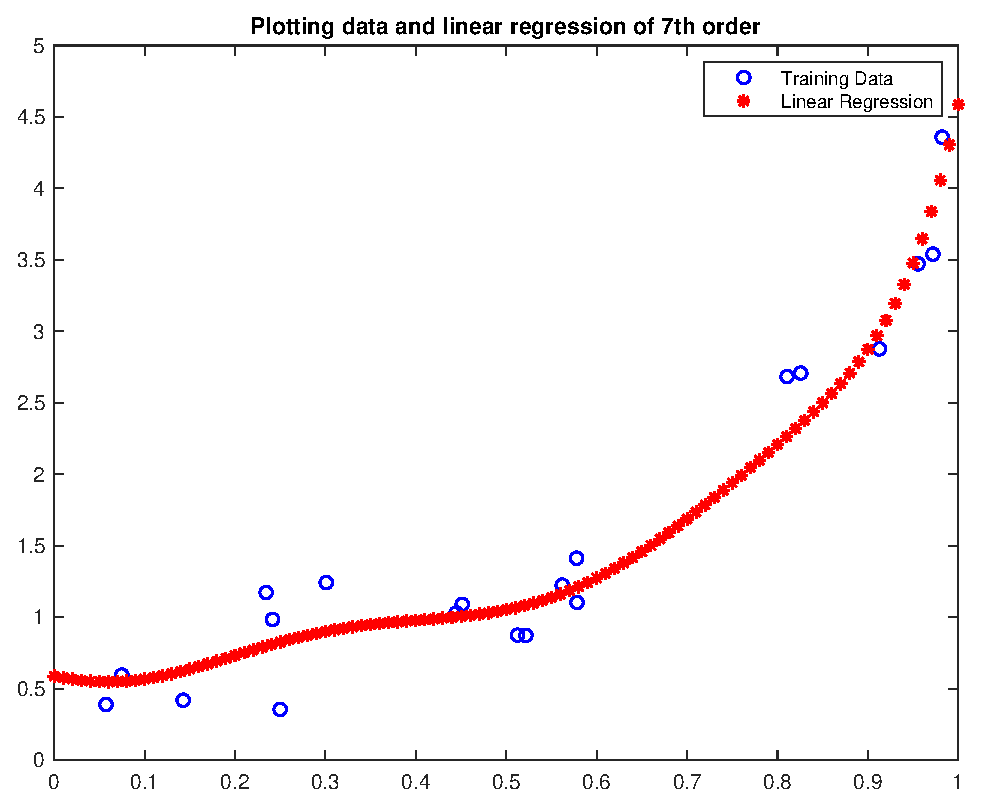
\includegraphics [width=4in]{practice1_05.eps}

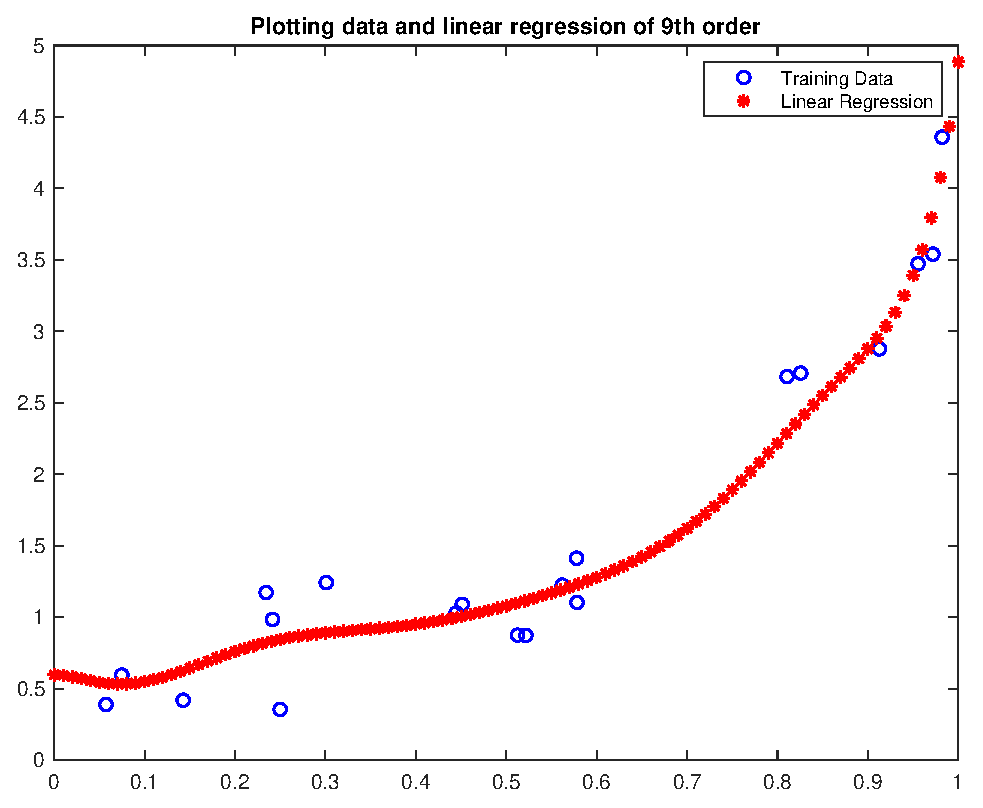
\includegraphics [width=4in]{practice1_06.eps}

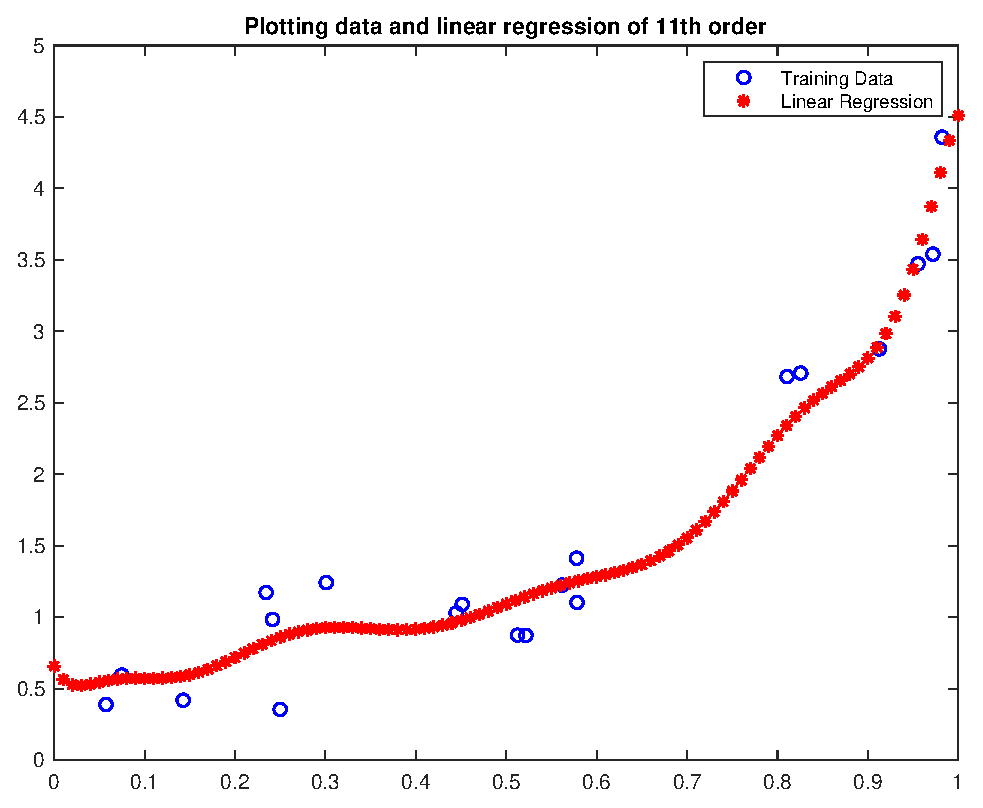
\includegraphics [width=4in]{practice1_07.eps}

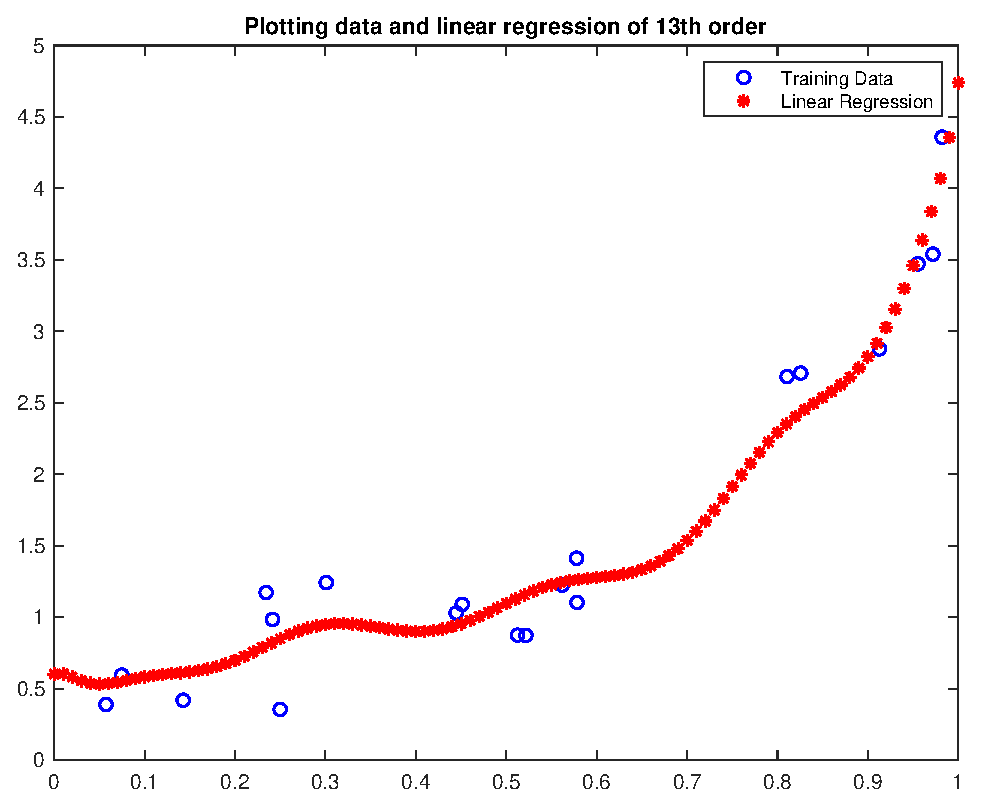
\includegraphics [width=4in]{practice1_08.eps}



\end{document}
    
